\chapter{Обзор предметной области}

Чтобы достичь намеченных целей, необходимо понять, что из себя представляет экран мобильного приложения, а также из каких элементов может состоять его интерфейс.

\section{Основные понятия}
В iOS существует различие между координатами, указываемыми в коде, и пикселями устройства \cite{pixel} -- наименьшими дискретными элементами двумерного цифрового изображения. 
Для большинства задач фактический размер точек \cite{point} не имеет значения, их цель -- обеспечить согласованный масштаб, который может использоваться в коде для указания размера и положения представлений и отображаемого содержимого. 
Например, если пиксели в два раза меньше изначальной высоты или ширины, можно использовать квадрат 2×2 пикселя для каждой точки (это называется масштаб @2x) -- рисунок \ref{fig:points}. 
Таким образом, измерение в точках позволяет корректно масштабировать изображение на экранах с высоким разрешением \cite{hig}.

\begin{figure}[h!]
	\centering{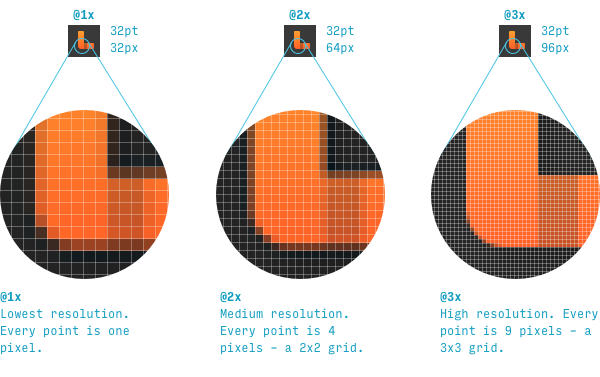
\includegraphics[scale=0.7]{img/point.png}}
	\caption{Точки и пиксели}
	\label{fig:points}
\end{figure}

Устройства, работающие на операционной системе iOS, имеют различное разрешение экрана и соотношение сторон. 
Так, например, iPhone X имеет разрешение 1125 x 2436 пикселей и коэффициент масштабирования в точки, равный 3.0 (то есть 375 x 812 точек), а iPhone 6  -- 750 x 1334 пикселей и коэффициент 2.0 соответственно (то есть 375 x 667) \cite{displays}. 
А также каждое устройство имеет горизонтальную и вертикальную ориентацию. 
Данные характеристики стоит учитывать в разработке, дабы создавать приложения, интерфейс которых адаптируется к устройствам разного размера, а также любой их ориентации. 

\section{UIKit}

UIKit \cite{uikit} -- библиотека, предоставляющая архитектуру окон и представлений для реализации пользовательского интерфейса, включая компоненты, которые можно использовать для построения базовой инфраструктуры приложения. 
Альтернативой выступает фреймворк SwiftUI \cite{swiftui}, предоставляющий не меньше возможностей, однако, будучи представленной в 2016 году, библиотека не смогла стать столь популярной в разработке. 
Поэтому целесообразным будет рассмотреть методы верстки UI-элементов, предоставляемых UIKit.


Рассмотрим базовые UI-элементы, предлагаемые фреймворком UIKit.

UIView (или представление) \cite{uiview} -- это фундаментальный блок пользовательского интерфейса приложения, а UIView-класс определяет поведение, общее для всех представлений. 
Объекты этого класса отображают содержимое в пределах своих границ и обрабатывают любые взаимодействия с этим содержимым. 
Для отображения надписей, изображений, кнопок и других элементов интерфейса, обычно встречающихся в приложениях, используют не определяемые самостоятельно подклассы view, а предоставляемые платформой UIKit. 

UIViewController (или контроллер) \cite{controller} -- объект, который управляет иерархией представлений приложения. Основные обязанности контроллера включают следующее:

\begin{itemize}[label=---]
	\item обновление содержимого представлений;
	\item реагирование на взаимодействие пользователя с представлениями;
	\item изменение размеров представлений и управление макетом общего интерфейса;
	\item координация с другими объектами, включая другие контроллеры представления.
\end{itemize}

Итак, экран в мобильной разработке представляет UIViewController, являющийся контейнером для других UIView. 
Труд команды разработки интерфейса мобильного приложения сводится к задаче корректного отображения элементов на экране -- расположения UIView на UIViewController. 
Чтобы работа была эффективной, целесообразно каждому члену команды дать индивидуальную подзадачу -- таким образом используемая технология верстки должна предполагать возможность работы нескольких участников над одним проектом и минимизировать количество ошибок, возникающих при изменении параметров UI-элементов. 

На основе рассмотренных теоретических сведений можно выделить критерии, по которым необходимо провести анализ эффективности использования методов верстки:

\begin{itemize}[label=---]
	\item возможность создания интерфейса, масштабируемого для устройств разного размера и двух ориентаций экрана, и относительная сложность его создания;
	\item возможность командной разработки интерфейса;
	\item сложность внесения изменений в интерфейс;
	\item возможность обработки всех параметров UI-элемента;
	\item скорость работы метода.
\end{itemize}

\chapter{Методы верстки}

Под понятием разметки подразумевается расчет необходимых координат и размеров UI-элементов.
Существует два основных подхода к созданию пользовательского интерфейса: можно программно компоновать элементы, задавая координаты и размеры каждого в коде, или же использовать автоматическую компоновку.

\section{Ручная верстка}

\subsection{Frame}

Frame \cite{frame} -- свойство view, описывающее прямоугольник, определяющий местоположение и размер представления в системе координат его родительского view \cite{superview}.

View, изображенную на рисунке \ref{fig:frame}, можно описать кодом, представленным в листинге \ref{lst:code1}. 

\begin{figure}[h!]
	\centering{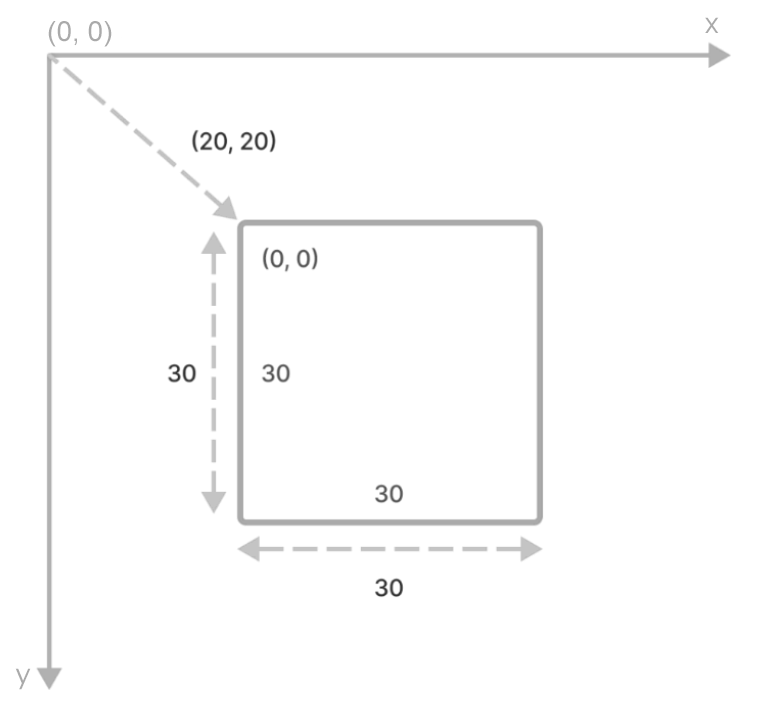
\includegraphics[scale=0.65]{img/frame.png}}
	\caption{Frame}
	\label{fig:frame}
\end{figure}

%\hspace{0.6cm}В Листинге представлен задание свойства frame для UIView.
\begin{lstlisting}[label=lst:code1, caption=Задание свойства frame для UIView]
	var view = UIView()
	view.frame = CGRect(x: 20, y: 20, width: 30, height: 30)
\end{lstlisting}

Ручная верстка предполагает задание кодом координат и размеров каждого элемента экрана. 
Указание координат идет относительно левого верхнего угла экрана -- именно там располагается точка (0, 0). 
При желании запустить будущее приложение на двух устройствах, размеры экрана которых различны, результат также будет разниться. 
То же будет происходить и при попытке сравнения экранов горизонтальной и вертикальной ориентации. 
Таким образом, возникает необходимость вручную обрабатывать каждый из возможных размеров дисплея в двух вариациях ориентации. 
На данный момент существует 10 различных размеров экрана iPhone и 7 -- iPad. 
Нетрудно представить, во сколько раз увеличивается количество строк кода и повышается трудоемкость задачи при обработке каждого случая. 

Однако данный подход позволяет разбить задачу создания интерфейса на несколько подзадач, поскольку в пределах одной superview разработчик взаимодействует лишь с этим родительским представлением и конкретной view. Внесение изменений в написанный раннее код также не составит большого труда, так как параметры, задаваемые в свойстве frame, независимы друг от друга, и их значения являются константами.

При использовании данного метода разметки разработчик получает возможность создания любого кастомного элемента, поскольку имеет доступ к обработке каждого визуального параметра UI-элемента. 
Так, например, можно задавать радиус угла view, цвет и прозрачность элемента, что представлено в листинге \ref{lst:code2}.

\begin{lstlisting}[label=lst:code2, caption=Задание параметров view]
	var view = UIView()
	view.frame = CGRect(x: 20, y: 20, width: 30, height: 30)
	view.layer.cornerRadius = 2.0
	view.backgroundColor = UIColor.red.withAlphaComponent(0.5)
\end{lstlisting}

Для того, чтобы оценить время работы метода, необходимо упомянуть, что любые модификации UI-элементов производятся на главном потоке многопоточного приложения -- main thread \cite{mainthread}. Поскольку параметрами свойства frame выступают константа, а, соответственно, никакие вычисления не производятся, скорость работы метода будет соответствовать скорости размещения элементов на экране. 


\section{Автоматическая верстка}

Существует альтернативный способ расчета необходимых координат и размеров. 

Автоматическая компоновка (или Auto Layout) \cite{autolayout} динамически вычисляет размер и положение всех видов в иерархии на основе ограничений, наложенных на эти view. Например, существует возможность ограничить кнопку так, чтобы она была центрирована по горизонтали в соответствии с видом изображения и ее верхний край всегда оставался на 8 точек ниже нижнего края изображения. 

Правила (или constraints), задаваемые Auto Layout, представляют собой обычное линейное уравнение вида \begin{equation}
	y = a \cdot x + b,
\end{equation}
где y – необходимая координата или размер; a – произвольный множитель; x – параметр, от которого зависит итоговый результат; b – константа. Для того чтобы корректно посчитать координаты и размер элемента, необходимо минимум 3 правила, которые сложатся в систему равнений, результатом решения которой будут координаты и размер элемента.

Существует два основных способа задать ограничения для автоматической компоновки: программный, когда каждое ограничение представлено строкой кода, и автоматический, когда ограничения заданы с помощью инструмента работы с пользовательским интерфейсом Interface Builder и Storyboard \cite{storyboard}.

\subsection{Auto Layout программно}

Автоматическая компоновка предоставляет возможность создавать масштабируемый для устройств разных размеров и ориентации экрана интерфейс, поскольку значения ограничений вычисляются динамически при внутренних или внешних изменениях. 

К внешним относятся изменение размера окна и вращение устройства.
К внутренним -- изменение содержимого, отображаемого приложением.

\begin{figure}[h!]
	\centering{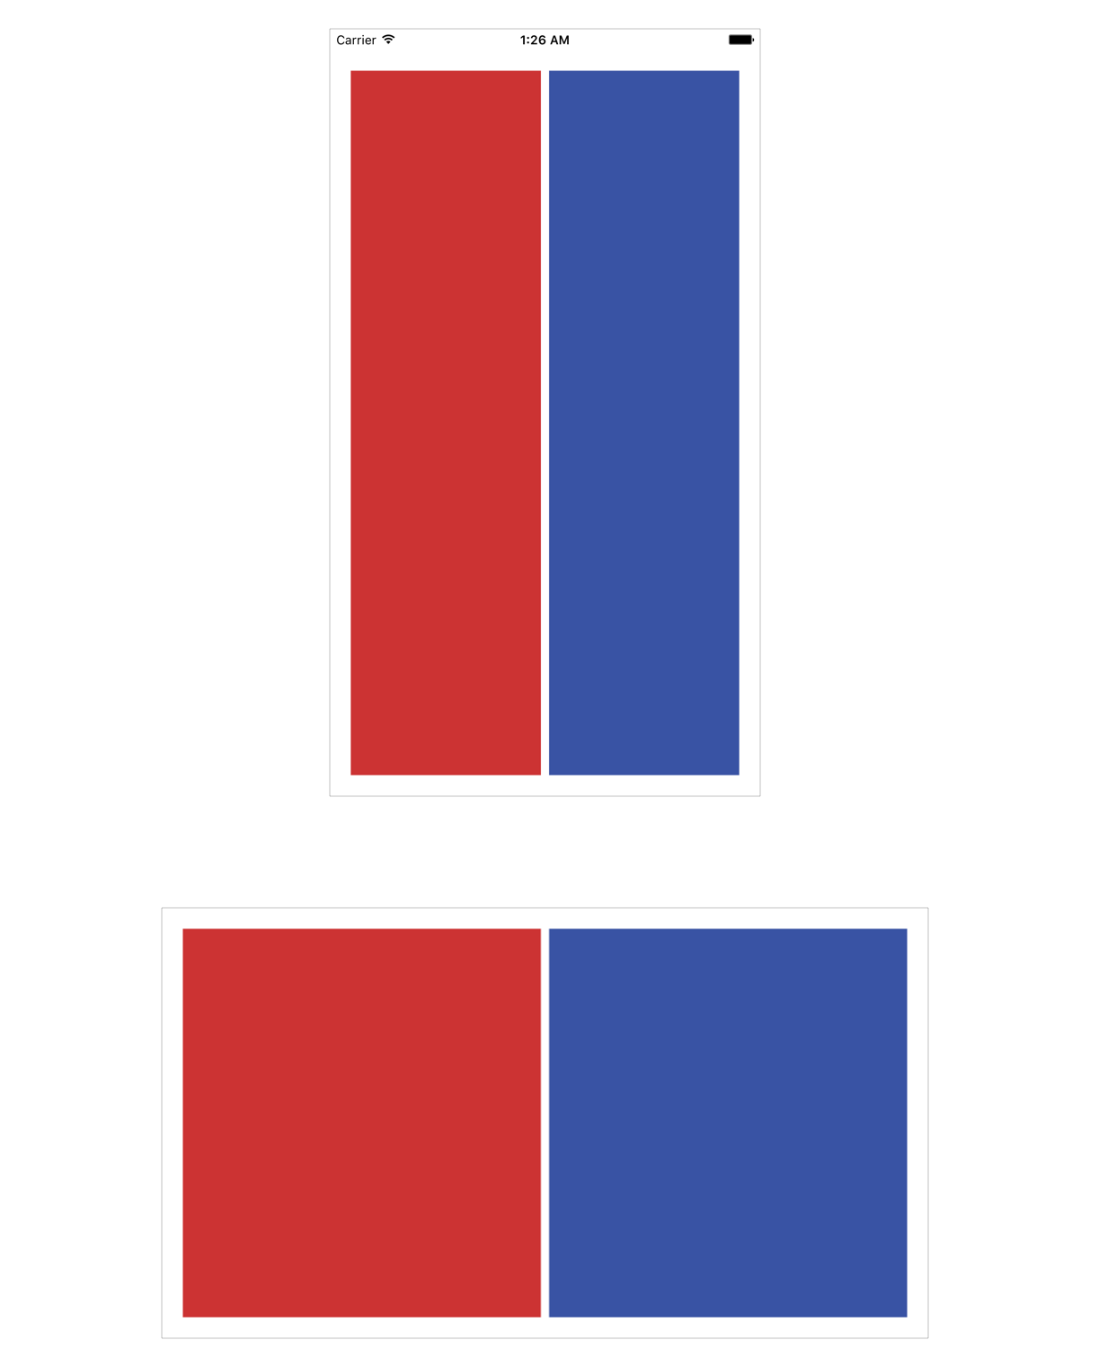
\includegraphics[scale=0.79]{img/autolayout.png}}
	\caption{UIView, скомпонованные с помощью Auto Layout}
	\label{fig:autolayout}
\end{figure}

Например, для расположения на экране двух UIView, находящихся справа и слева друг от друга, как представлено на рисунке \ref{fig:autolayout}, можно использовать ограничения, представленные в листинге \ref{lst:code3}.

\newpage

\begin{lstlisting}[label=lst:code3, caption=Задание параметров view]
// Vertical Constraints
Red.top = 1.0 * Superview.top + 20.0
Superview.bottom = 1.0 * Red.bottom + 20.0
Blue.top = 1.0 * Superview.top + 20.0
Superview.bottom = 1.0 * Blue.bottom + 20.0
 
// Horizontal Constraints
Red.leading = 1.0 * Superview.leading + 20.0
Blue.leading = 1.0 * Red.trailing + 8.0
Superview.trailing = 1.0 * Blue.trailing + 20.0
Red.width = 1.0 * Blue.width + 0.0
\end{lstlisting}

Строки кода позволяют проследить логику задания ограничений, поэтому внесение изменений в уже описанный интерфейс не является сложной задачей: необходимо лишь понимание того, какие модификации претерпевает UI-элемент на каждом этапе наложения на него ограничений. Из чего вытекает возможность и командной разработки с использованием метода Auto Layout.

Также сохраняется возможность создания любого кастомного элемента, поскольку доступ к обработке каждого визуального параметра UI-элемента все еще доступен при программной верстке.

Основной проблемой при автоматическом расчете разметки является скорость работы. При увеличении
количества правил усложняется система уравнений, которая должна быть решена чтобы были получены все координаты и размеры. Так как этот механизм является закрытой системой, то программист не может повлиять на скорость работы алгоритмов. К тому же все расчёты производятся в главном потоке приложения: например, при наличии в интерфейсе списка со сложными элементами и быстром его прокручивании расчет всех координат и размеров будет занимать очень много времени, что в итоге скажется на плавности прокручивания.


\subsection{Interface Builder}

Interface Builder \cite{interfacebuilder} представляет собой инструмент для создания пользовательского интерфейса: сцена, на которую можно перетаскивать view из библиотеки видов -- рисунок \ref{fig:builder}. 
Программист имеет возможность настраивать ограничения, выравнивать и закреплять каждый UI-элемент с помощью всплывающих окон. 

\begin{figure}[h!]
	\centering{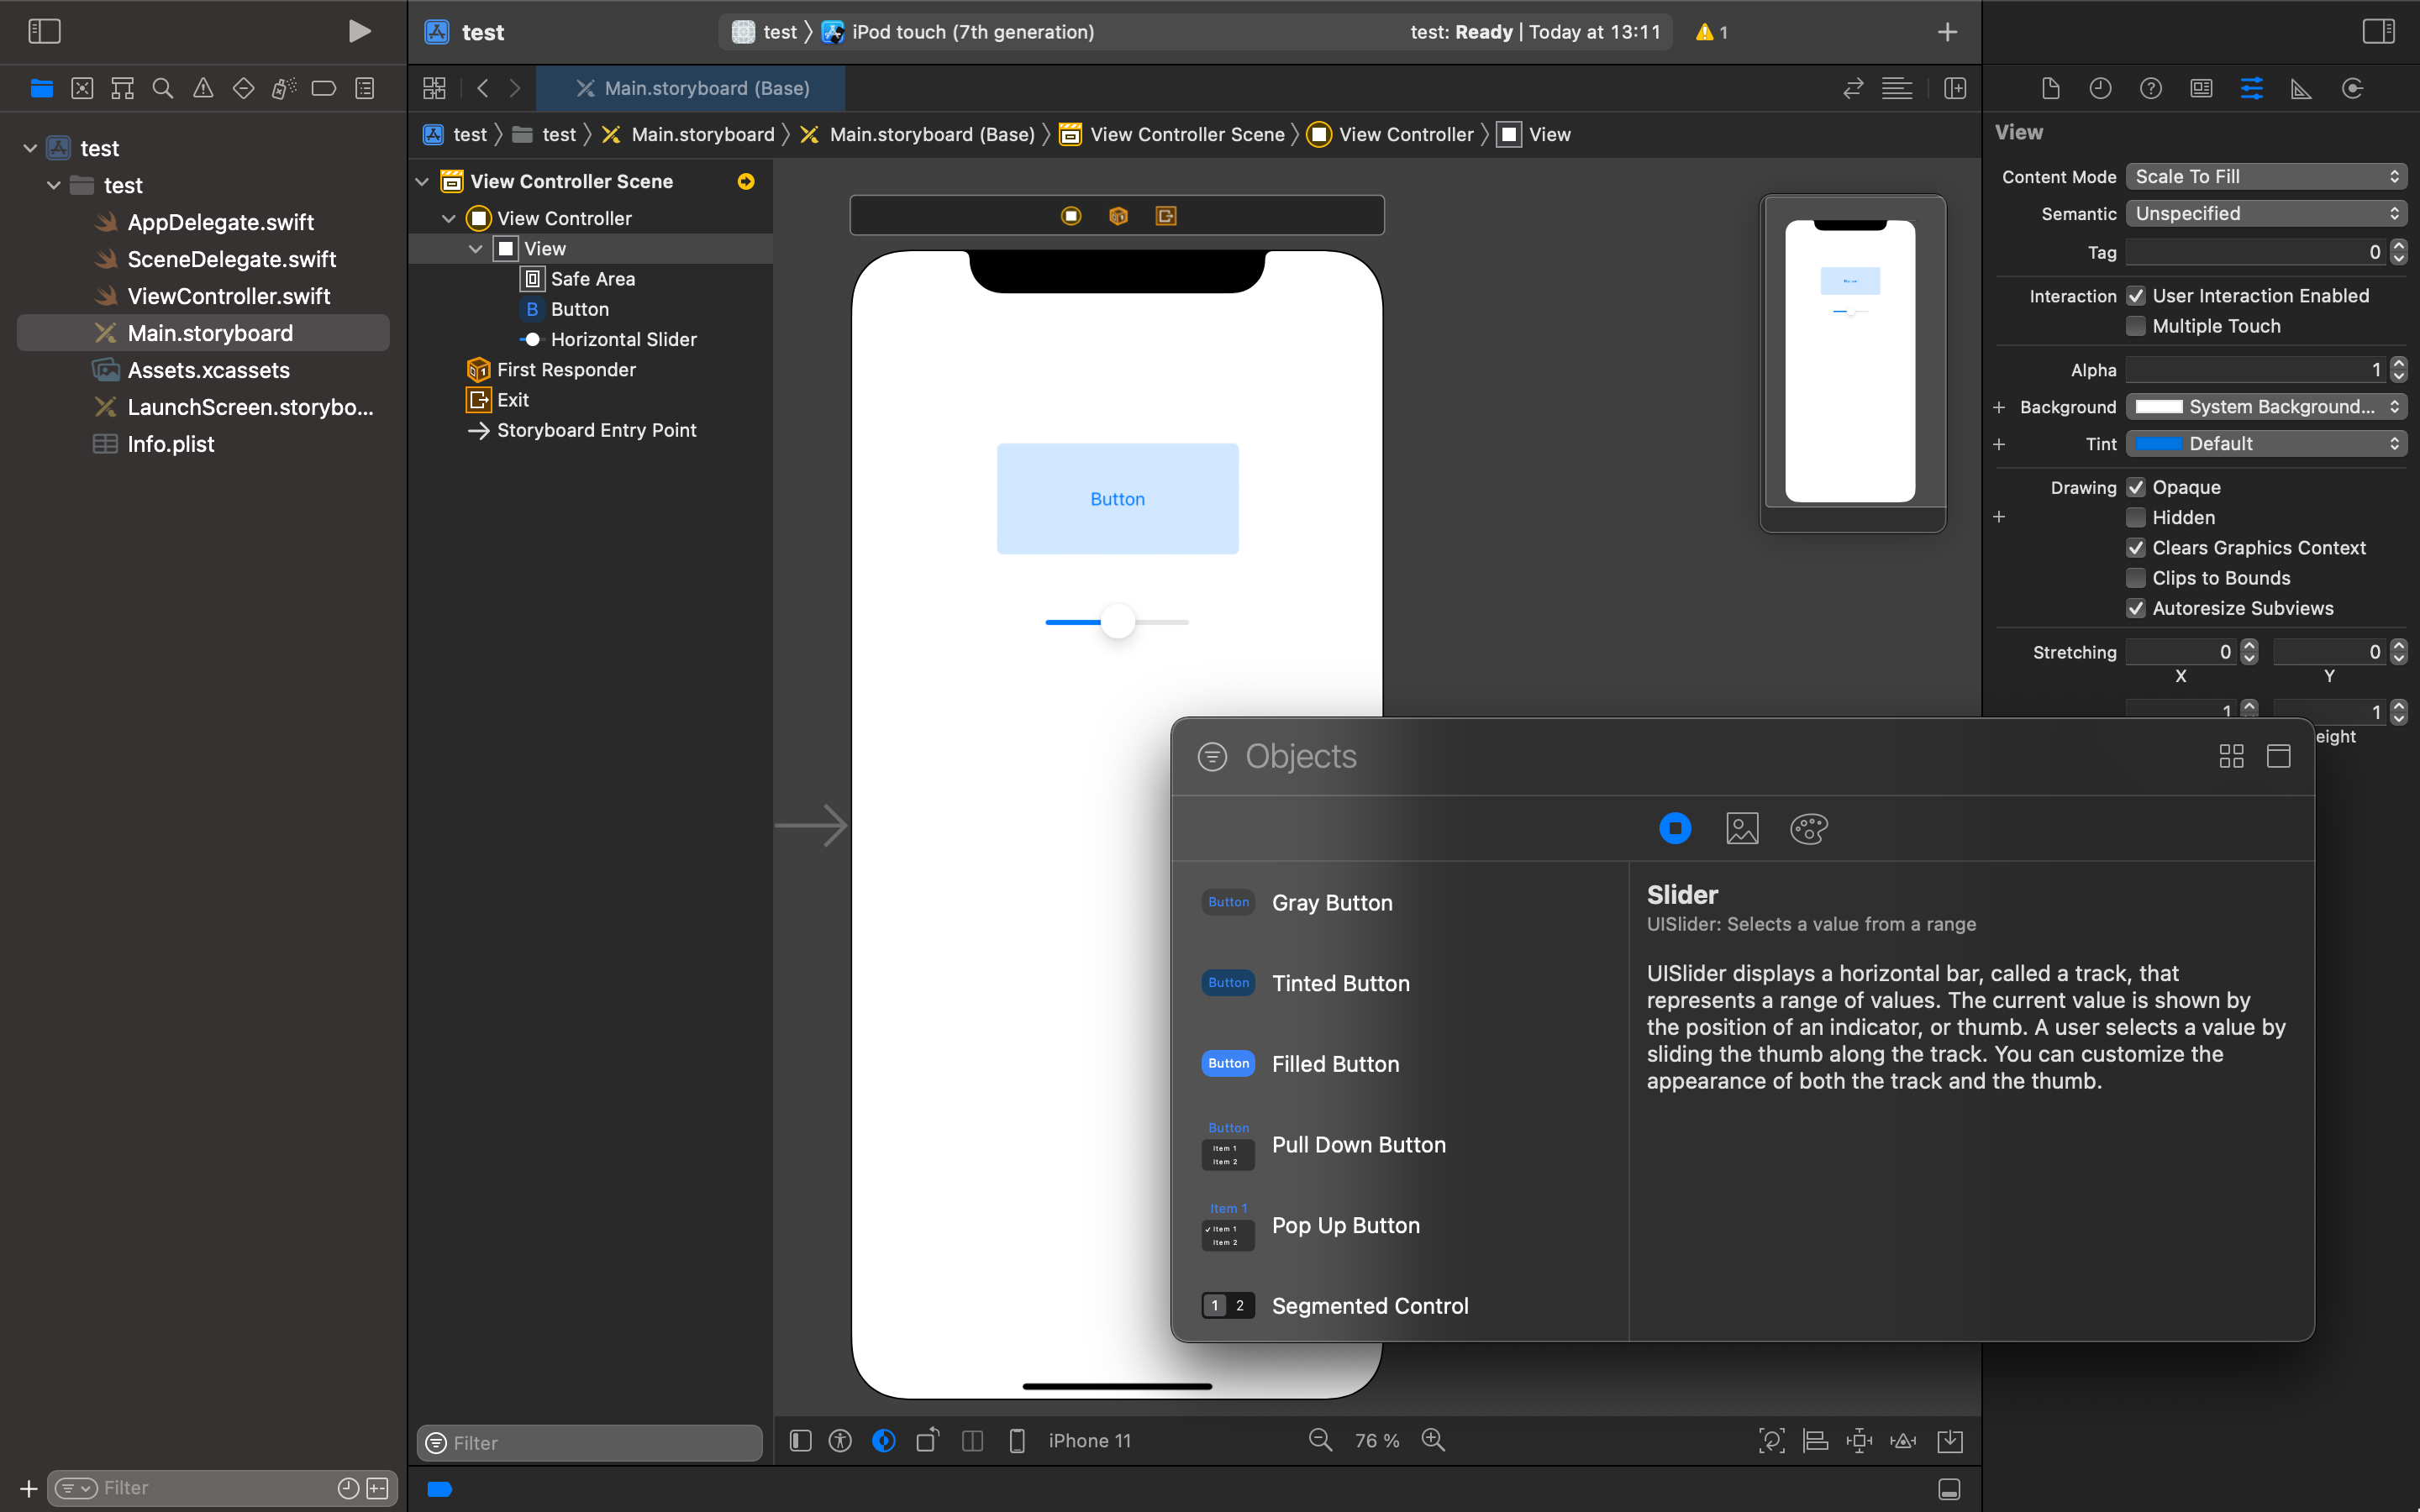
\includegraphics[scale=0.30]{img/builder.png}}
	\caption{Interface Builder}
	\label{fig:builder}
\end{figure}

Таким образом, интерфейс может быть создан без написания кода. 
Однако если в одних случаях это является бесспорным преимуществом, в других -- источником проблем или грозит отсутствием возможности реализации всех задумок.

Этот метод верстки имеет преимущество в разработке статического интерфейса небольшого приложения: при его создании существенно сократится время разработки, поскольку больше не нужно каждое ограничение для UI-элемента описывать строкой кода. 
Также имеется возможность легко изменять параметры какого-либо конкретного элемента: например, длину лэйбла. 
Однако Interface Builder не предоставляет возможности в динамике обрабатывать изменения интерфейса, а также при большом количестве частей интерфейса сцена разрастется настолько, что перестает быть наглядной. 
Из чего вытекает, что внесение изменений в уже готовые проекты является сложной задачей, поскольку разработчик не имеет наглядно представленных правил ограничения UI. 
Следствием является и сложность командной разработки: сцена Interface Builder неделима, невозможно по отдельности обработать каждый UIView, закрепляемый на ней.

Невозможно обработать и каждый параметр UIView или слоя представления, так как рассматриваемый инструмент предоставляет лишь ограниченный список настраиваемых параметров. 
Так, например, разработчик не имеет возможности задать view, края которой скруглены, из Interface Builder.

Затраты по времени метода зависят от сложности сцены: чем объемнее сцена, тем больше времени требует процессор для обработки графических элементов, расположенных на ней, и преобразования в код. 


